\chapter{Raccolta dati ed analisi}
\vspace{0.5cm}
\label{cha:789}

Analizzando i diversi comportamenti della droplet nei vari esperimenti eseguiti e tenendo in considerazione che l'obiettivo di tale studio è quello di fare in modo che questa si muova velocemente e in maniera precisa lungo un percorso ipotizzato, si è cercata la combinazione ``migliore" dei parametri sperimentali che permettesse alla droplet di avvicinarsi il più possibile e nel minor tempo al punto in cui il sale è stato posto. Lo studio di questo movimento di chemiotassi, ci aiuterà a comprendere e a riprodurre le dinamiche di movimento delle cellule viventi.

\section{Esperimento con software}
L'esperimento precedentemente descritto, è stato eseguito per mezzo del programma appositamente sviluppato, utilizzando le API di EvoBot e sfruttando funzioni avanzate della libreria OpenCV. Per portare a termine l'intero esperimento, occorre completare tre fasi: preparazione, raccolta dati, elaborazione dati. 

\subsection{Preparazione}
Per permettere al robot di accedere a liquidi e risorse esterne, bisogna posizionare sul piano degli esperimenti tutto ciò di cui si potrebbe avere bisogno. Seguendo lo schema in figura, si posiziona (A) il decanolo, (B) il sale e (C) la Petri dish contenente uno strato di Decanoato.
\begin{figure}[h]
	  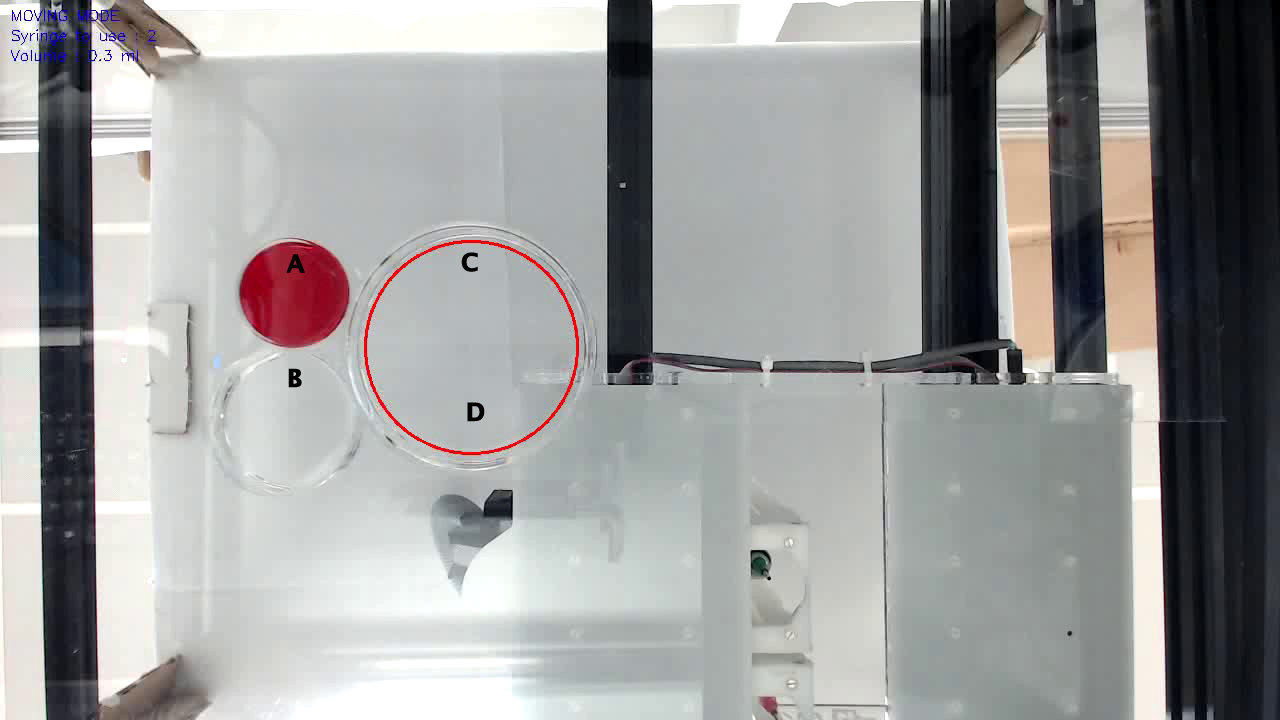
\includegraphics[scale=0.30]{immagini/exp1.jpg}
		\centering
	 \caption{experimental layout}
	\end{figure} 
\\Il protocollo seguito prevede cinque passaggi fondamentali: 
\begin{enumerate}

	\item Limitare l'area di interesse.\\
		La necessità di utilizzare Petri dish di diametri differenti e i problemi che possono essere causati da molteplici agenti esterni hanno suggerito che limitare la zona di interesse per ogni singolo esperimento potesse essere una soluzione: attraverso l'apposita interfaccia è possibile, quindi, disegnare un cerchio attorno alla Petri dish. Tutto ciò che si trova all'esterno di questo limite virtuale non verrà considerato dal programma.

	\item Prelevare $50\mu L$ di decanolo.\\
		Utilizzando una siringa delle due a disposizione, si raggiunge il pozzetto A, si fa scendere il corpo della stessa per prelevarne la quantità di decanolo richiesta. Bisogna tenere in considerazione che l'unità di volume che si può gestire è di $10\mu L$, grandezza nata dal compromesso tra avere un'interfaccia utilizzabile e una precisione accettabile. 

	\item Rilasciare $30\mu L$ di decanolo.\\
		 Posizionando la siringa precedentemente caricata sopra la Petri dish in poszione C, si rilascia il decanolo. 
La scelta di prelevare una quantità maggiore di quella richiesta ci assicura l'immissione nel sistema della corretta quantità in quanto può accadere che un volume non definito venga trattenuto nel corpo o nella punta della siringa.

	\item  Prelevare $500\mu L$ di NaCl. \\
		Utilizzando l'altra siringa, si raggiunge il pozzetto B e si eseguono le stesse azioni del punto 2, prelevando questa volta il sale. 
	
	\item Immettere $200\mu L$ di NaCl.\\
		Posizionando la siringa attualmente in uso sopra la Petri dish in posizione D, si rilascia il sale. 
\end{enumerate}

\subsection{Raccolta dati}
Fino ad ora l'utilizzo di EvoBot potrebbe risultare superfluo, è in questa fase che si può percepire il valore aggiunto che una macchina riesce ad apportare. Tramite l'utilizzo della webcam statica e la libreria di OpenCV, il programma permette di tracciare passo-passo i movimenti della droplet, fino a 30 movimenti al secondo. Avere a disposizione i singoli punti dell'intero tracciato, permette di registrare qualsiasi particolare caratteristica che sarebbe sfuggita all'occhio umano. L'utilizzo che si  può fare di questi punti è limitato solo dalla fantasia, si possono calcolare accelerazioni, \emph{pattern} oppure si possono comparare più percorsi dello stesso esperimento.
\\Nel nostro caso ci siamo limitati ad osservare se ci fosse un movimento della droplet verso il sale e si è cercato di capire in che ambiente questo risultasse più veloce e più preciso.
\\Per permettere alla webcam di riconoscere la droplet, questa è stata colorata di rosso grazie all'aggiunta del colorante Oil Red O alla soluzione di decanolo. Tuttavia, le droplet possono essere colorate non solo di rosso ma anche di altri colori, a seconda delle esigenze. Il programma mette a disposizione alcuni dei colori più utilizzati (come il rosso, il verde e il blu). 
\\ Per estrapolare informazioni dai dati raccolti durante l'esperimento, il programma si serve del salvataggio di essi su di un file \emph{.csv}.
Un esempio di questo file è disponibile nella tabella sottostante. 

\begin{center}
\begin{tabular}{lllllll}
X salt & Y salt & X droplet Start & Y droplet Start & X droplet End & Y droplet End & time(s) \\
\hline
405    & 418    & 378             & 300             & 425           & 434           & 88  
\end{tabular}
\end{center}


\subsection{Elaborazione dati}
I file prodotti durante la raccolta dati, vengono successivamente presi in carico da un altro programma che ha il compito di analizzare queste rilevazioni col fine di generare un unico file contenente dati e metadati dei singoli esperimenti.
\\La colonna più importante del file generato è quella che prende il nome di ``k". Questo coefficiente indica la precisione con cui la droplet si avvicina al sale ed è definita come:
\begin{equation} 	
	k := \frac { d(C,B) }{ d(A,C) }
\end{equation}
Dove A rappresenta il punto in cui la droplet viene trovata all'inizio del tracking , B quello in cui viene posizionato il sale, C dove la droplet si trova ad esperimento concluso, $d$ calcola la distanza euclidea tra i punti in questione. 
\\Possiamo assumere che più $d(C,B)$ tende a zero, più l'esperimento è preciso; da questo si evince che avere un $k$ tendente a zero è indice di successo.   
\begin{figure}[h]
	  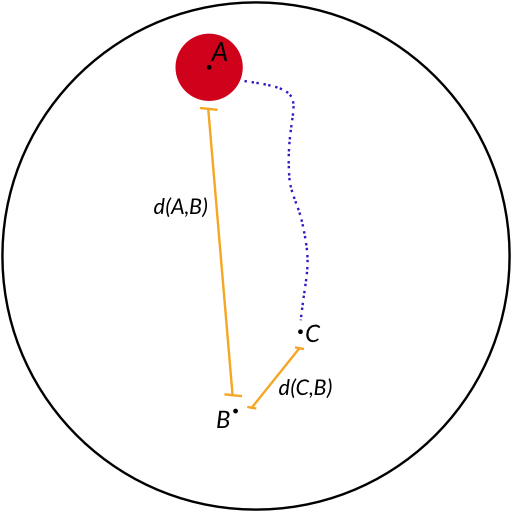
\includegraphics[scale=0.30]{immagini/schema.png}
		\centering
	 \caption{schema di un esperimento e degli elementi analizzati}
\end{figure} 
Una volta ottenuti tutti i $k$, mantenendo costante il $pH$ e le molarità, si vanno a calcolare tutti i $k$ medio per ogni singolo ambiente. L'ambiente rappresentato dal minor $k$ medio è quello che permette alla droplet di raggiungere il sale in maniera precisa e veloce. 
\\Durante la raccolta dati si è deciso di salvare anche il tempo impiegato dalla droplet nel movimento ma questo dato non viene utilizzato in questo studio e potrà essere analizzato in studi futuri. 

\section{Risultati}
La soluzione di acido decanoico presente nella Petri prima dell'inizio dell'esperimento si presenta sottoforma di ione decanoato con carica negativa. Per disciogliere 20mM di acido decanoico in $1L$ di acqua abbiamo bisogno di aumentare il pH altrimenti l'acido resterebbe in forma solida. I risultati sono stati suddivisi per classi di molarità per rendere più semplice la lettura dei dati.

\subsection{20mM}
Nelle figure seguenti si osservano le droplet nelle tre condizioni differenti di pH. Nella soluzione di Decanoato con $pH11$ la droplet percorre un tratto più lungo rispetto alle altre con pH maggiori e inoltre sono distinguibili il punto di inizio e il punto di fine. Per le altre due soluzioni non si può dire lo stesso, infatti i punti di inizio e fine del percorso risultano, se non coincidenti, molto vicini. 
\begin{figure}[h]
	\centering
   		{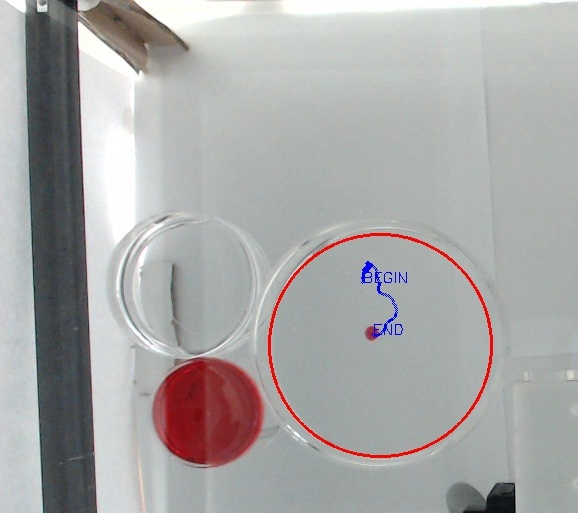
\includegraphics[width=5cm]{immagini/20mMpH11-2.jpg}} %ph11
 	\hspace{2mm}   	
		{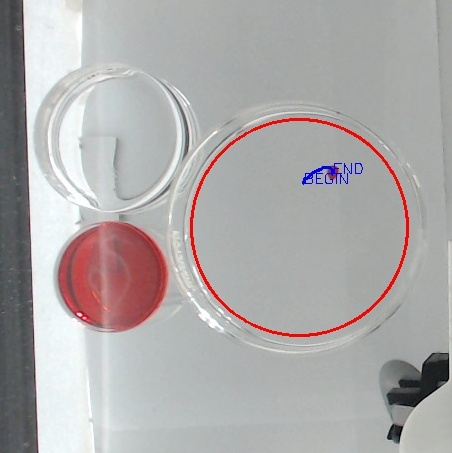
\includegraphics[width=5cm]{immagini/20mMpH12-2.jpg}}%ph12
	\hspace{2mm}   	
		{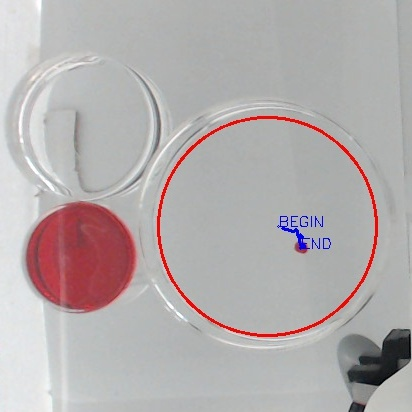
\includegraphics[width=5cm]{immagini/20mMpH13-2.jpg}}%ph13
	\caption{Acido decanoico 20mM a pH11, 12 e 13}
\end{figure}
\\Nelle soluzioni con molartità $20mM$ si osserva, per tutti e tre i pH analizzati, che la droplet compie dei percorsi brevi come se l'alta concentrazione di Decanoato fornisse un ostacolo ad un movimento più lineare e complesso. 
\\Nella tabella 4.1 sono riportati i valori del coefficiente $k$ per ogni esperimento eseguito ed i valori medi accanto. Come osservato dalle immagini raccolte, la soluzione con $pH11$ risulta avere il coefficiente medio minore, per cui il movimento può essere considerato il migliore.  
\begin{table}
\caption{Valori del k e valori medi per ogni classe di pH delle soluzioni $20mM$}
\begin{center}
\begin{tabular}{ll}
pH & k     \\
11 & 0,573 \\
11 & 2,429 \\
11 & 1,458 \\
11 & 3,594 \\
12 & 4,075 \\
12 & 3,329 \\
12 & 3,284 \\
12 & 2,742  \\
13 & 2,236 \\
13 & 2,932 \\
13 & 5,231 \\
13 & 8,571
\end{tabular}
\begin{tabular}{ll}
pH & k medio \\
11 & 2,013  \\
12 & 3,357   \\
13 & 4,742
\end{tabular}
\end{center}
\end{table}
\pagebreak
\subsection{10mM}
Nelle seguenti figure si osservano i percorsi della droplet in soluzioni con molarità $10mM$ di Decanoato, per ogni classe di pH. Si osserva subito che i percorsi risultano più lunghi degli esperimenti precedenti ed in tutti e tre i casi si possono distinguere con chiarezza i punti di inizio e di fine percorso. 
\begin{figure}[h]
	\centering
   		{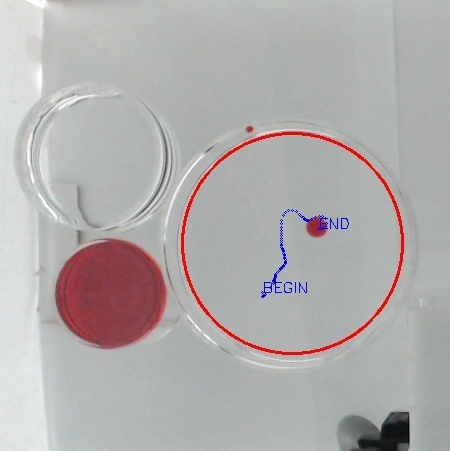
\includegraphics[width=5cm]{immagini/10mMph11-2.jpg}} %ph11
 	\hspace{2mm}   	
		{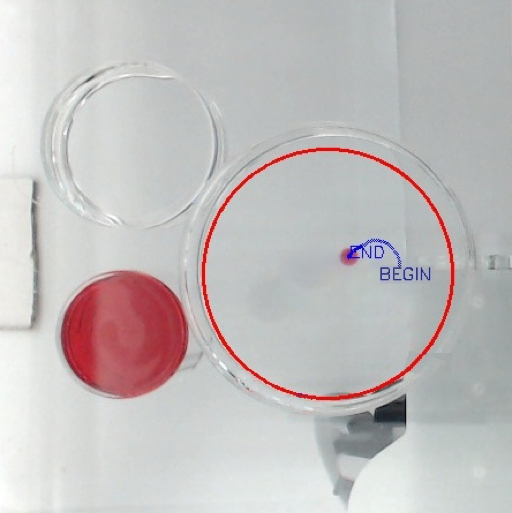
\includegraphics[width=5cm]{immagini/10mMpH12-1.png}} %PH 12
	\hspace{2mm}   	
		{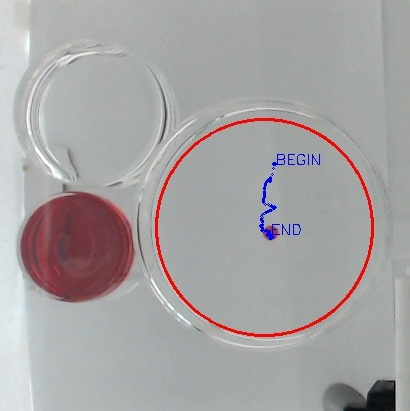
\includegraphics[width=5cm]{immagini/10mMpH13-2.jpg}}  %PH 13
	\caption{Acido decanoico 10mM a pH11, 12, 13}
\end{figure}
\\Nella tabella 4.2 vengono riportati i valori di $k$ e i valori medi per ogni classe di pH. Si osserva, anche in questo caso, che la soluzione con $pH11$ rivela il risultato migliore. 
\begin{table}
\caption{Valori del k e valori medi per ogni classe di pH delle soluzioni $10mM$}
\begin{center}
\begin{tabular}{ll}
pH & k       \\
11 & 0,671   \\
11 & 0,074   \\
11 & 0,538   \\
11 & 0,209   \\
12 & 0,566   \\
12 & 0,241   \\
12 & 0,763   \\
12 & 0,447   \\
13 & 0,876   \\
13 & 0,338   \\
13 & 0,732   \\
13 & 0,424   
\end{tabular}
\begin{tabular}{ll}
pH & k medio \\
11 & 0,373   \\
12 & 0,504 \\
13 & 0,592
\end{tabular}
\end{center}
\end{table}
\pagebreak

\subsection{5mM}
Nell'ultima classe di molarità si osservano dei percorsi lunghi e lineari. Nelle soluzioni con $pH11$ e $pH13$ la droplet compie un percorso preciso e direzionale, nella soluzione a $pH12$ tuttavia, il percorso è più breve. Questo può essere dovuto a fattori esterni che posso aver influenzato l'esperimento.
\begin{figure}[h]
	\centering
   		{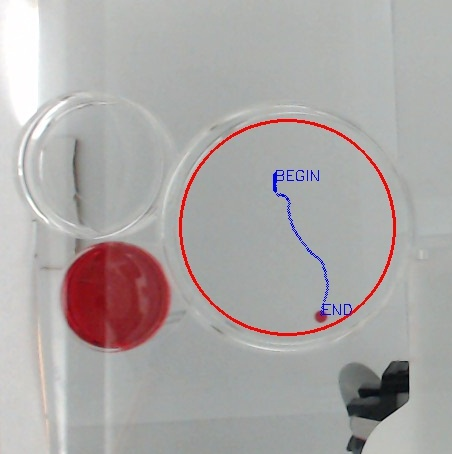
\includegraphics[width=5cm]{immagini/5mMpH11-1.jpg}} %ph11
 	\hspace{2mm}   	
		{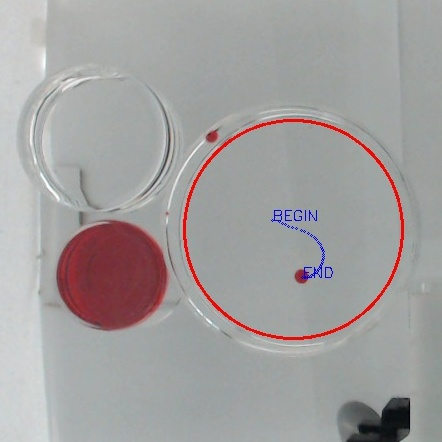
\includegraphics[width=5cm]{immagini/5mMpH11-2.jpg}}%ph12
	\hspace{2mm}   	
		{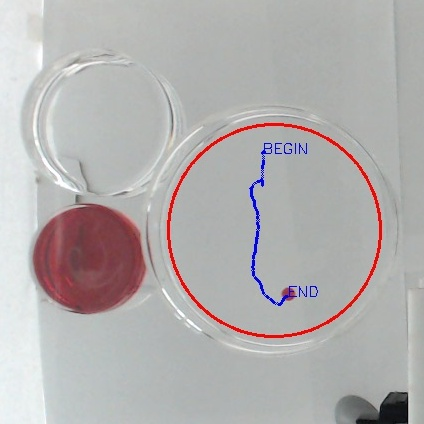
\includegraphics[width=5cm]{immagini/5mMpH13-2.jpg}}%ph13
	\caption{Acido decanoico 5mM a pH11, 12 e 13}
\end{figure}
\\Nella tabella 4.3 vengono riportati i valori di $k$ ed i valori medi per ogni classe di pH. Questi valori, comparati a quelli delle tabelle precedenti risultano i più bassi. Infatti gli spostamenti compiuti nelle soluzioni con molarità $5mM$ sono i più precisi.
\begin{table}
\caption{Valori del k e valori medi per ogni classe di pH delle soluzioni $5mM$}
\begin{center}
\begin{tabular}{ll}
pH & k       \\
11 & 0,18    \\
11 & 0,25    \\
11 & 0,213   \\
11 & 0,194   \\
12 & 1,837   \\
12 & 0,204   \\
12 & 0,393   \\
12 & 0,246   \\
13 & 0,171   \\
13 & 0,474   \\
13 & 0,289   \\
13 & 0,375   \\
\end{tabular}
\begin{tabular}{ll}
pH & k medio \\
11 & 0,209 \\
12 & 0,67    \\
13 & 0,327
\end{tabular}
\end{center}
\end{table}
\pagebreak

\subsection{Considerazioni generali}
In tutti gli esperimenti è stato notato che la droplet non risponde con il movimento chemiotattico immediatamente dopo l'aggiunta del sale. Probabilmente questo periodo di latenza è il tempo che il gradiente del sale impiega a raggiungere la droplet dal punto in cui è stato inserito.
Dopo questo periodo di latenza si è osservato un movimento agitatorio iniziale nel primo punto in cui la droplet viene riconosciuta dal tracking. Questo movimento oscillatorio può essere dovuto alla prima interazione tra il sale e le linee di confine della droplet.
Si è inoltre osservato, una volta che la droplet si avvicina al punto in cui è stato inserito il sale, che questa compie un movimento locale casuale ed oscillatorio, simile a quello compiuto al momento della prima interazione con il sale.
Nelle soluzioni con molarità $10mM$ e $5mM$ la droplet compie dei percorsi più lunghi, arrivando molto vicina al punto di inserimento del sale.  Tuttavia, nelle soluzioni con molarità $20mM$ si osservano dei movimenti più brevi, è come se la droplet facesse fatica a riconoscere il gradiente del sale compiendo un movimento minimo. Bisogna tenere in considerazione che questo movimento può essere stato influenzato da flussi di aria che hanno creato dei moti convettivi all'interno del sistema. I moti possono aver agito come forza contraria alla direzione del movimento. Un altro fattore esterno che ha portato alla creazione di moti convettivi può essere stato l'inserimento della punta della siringa all'interno della superficie dell'acido decanoico nella Petri. Tuttavia queste ipotesi potranno essere confermate attraverso la ripetizione di un maggior numero di esperimenti.
\begin{table}[h]
\caption{Tabella riassuntiva}
\begin{center}
\begin{tabular}{llll}
\textbf{ph}                       & \textbf{11}                         & \textbf{12}    & \textbf{13}    \\
\textbf{molarità}                 &                            &       &       \\
\textbf{20mM}                     & 2,013                      & 3,357 & 4,742 \\
\textbf{10mM}                     & 0,373                      & 0,504 & 0,592 \\ \cline{2-2}
\multicolumn{1}{l|}{\textbf{5mM}} & \multicolumn{1}{l|}{0,209} & 0,67  & 0,327 \\ \cline{2-2}
\end{tabular}
\end{center}
\end{table}
\\Nella tabella riassuntiva 4.4 sono stati raccolti tutti i valori medi di ogni combinazione. Come si può osservare il coefficiente di precisione migliore si ha nella soluzione di molarità $5mM$ con $pH11$. Inoltre, le soluzioni con molarità $20mM$ hanno i coefficienti maggiori tra tutte.














